\documentclass[a4paper]{report}
\usepackage{hyperref}
\usepackage{lastpage}
\usepackage{fancyhdr}
\usepackage{lineno}
\usepackage{listings}
\usepackage{german}
\usepackage[utf8]{inputenc}
\usepackage{amssymb}
\usepackage{graphicx}
\usepackage{tikz}
\usepackage{pgfgantt}
\usetikzlibrary{automata}
%\newcommand{\genasso}[2]{\begin{minipage}{0.7\textwidth}\begin{normalsize}\begin{flushleft}\textbf{{#1}}\end{flushleft}\end{normalsize}\vspace{-1cm}\begin{flushleft}\begin{small}{#2}\end{small}\end{flushleft}\end{minipage}\\\vspace{0.2cm}}
\pagenumbering{arabic}

\pagestyle{fancy} 
\newcommand{\frontmatter}{\clearpage \cfoot{\thepage\ }
\setcounter{page}{1}
\pagenumbering{Roman}}
\newcommand{\mainmatter}{\clearpage \lhead{\myAuth} \rhead{\myDate} \cfoot{} \rfoot{\thepage\ of \pageref{LastPage}}
\setcounter{page}{1}
\pagenumbering{arabic}}
\newcommand{\backmatter}{\clearpage \rfoot{\thepage\ }
\setcounter{page}{1}
\pagenumbering{alph}}


\newcommand{\makemytitlepage}{\begin{titlepage}
    \begin{center}
        \vspace*{0.8cm}
        
        \Huge
        \textbf{\myTitle}
        
        \vspace{1.5cm}
        
        \Large
        \myAuthor

        \vspace{1.8cm}

        %\begin{large}\textbf{Abstract:} \myAbstract \end{large}
        \includegraphics[width=6cm]{./IM.jpg}  
        
        \vfill
        
        \huge
        \myAsso
        
        \vspace{1.3cm}
        
        \Large

        \myDate
        
    \end{center}
\end{titlepage}}
\newcommand{\myAuth}{Team: *Iron Man*\\B. Pohl, K. Trogant, R. Enseleit, D. Hebecker}
\newcommand{\myAuthor}{Birgit Pohl 574353 (MO. 9-11)\\Kevin Trogant 572451 (Mo. 15-17)\\Ronja Enseleit 572404 (Mo. 15-17)\\Dustin Hebecker 571271 (MO. 9-11)}
\newcommand{\myAsso}{Group: *Iron Man*}
\newcommand{\myDate}{\today}

%%%%%%%%%%%%%%%%%%%%%%%%%%%%%%%%
%%Change Title !!!!!!!!!!!!!!!!!
%%%%%%%%%%%%%%%%%%%%%%%%%%%%%%%%
\newcommand{\myTitle}{Exercise Sheet 1}

\begin{document}
\frontmatter
\makemytitlepage
\mainmatter

%%%%%%%%%%%%%%%%%%%%%%%%%%%%%%%%%%%%%%%%%%%%%%%%%%%%%%%%%%
%% Only modify below here  and change myTitle!!!!!!!!!!!!!
%%%%%%%%%%%%%%%%%%%%%%%%%%%%%%%%%%%%%%%%%%%%%%%%%%%%%%%%%%
\section*{Aufgabe 1 (Program Evaluation and Review Technique)}
\subsection*{a)}
% Anyone good with TikZ?
%  https://www.youtube.com/watch?v=LoBC8zIB-3k
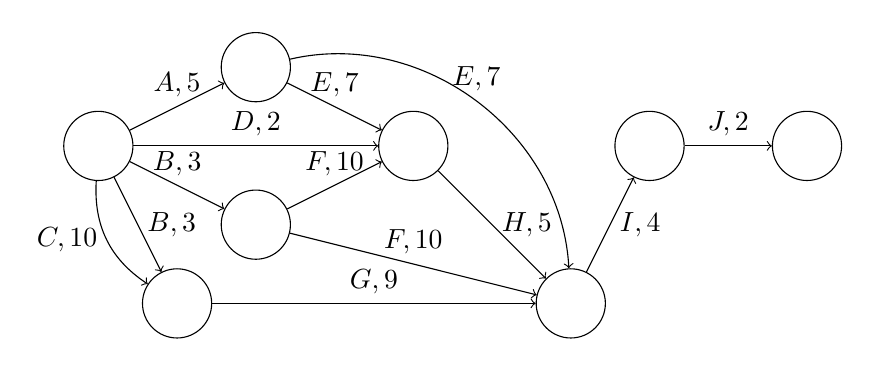
\begin{tikzpicture}[node distance=4cm]
	\node (a) at (0, 2) [state] {};
	\node (b) at (2, 3) [state] {};
	\node (c) at (4, 2) [state] {};
	\node (d) at (2, 1) [state] {};
	\node (e) at (1, 0) [state] {};
	\node (f) at (6, 0) [state] {};
	\node (g) at (7, 2) [state] {};
	\node (h) at (9, 2) [state] {};
	
	\path[->]
		(a) edge node[above] {$A, 5$} (b)
		(b) edge node[above] {$E, 7$} (c)
		(a) edge node[above] {$D, 2$} (c)
		(a) edge node[above] {$B, 3$} (d)
		(d) edge node[above] {$F, 10$} (c)
		(a) edge node[right] {$B, 3$} (e)
		(a) edge[bend right] node[left] {$C, 10$} (e)
		(e) edge node[above] {$G, 9$} (f)
		(c) edge node[right] {$H, 5$} (f)
		% One cold argue, that it's kind of pointless to include dependencies twice (eg. by depending on H (which depends on E) and E).
		(b) edge[bend left=50] node[above] {$E, 7$} (f)
		(d) edge node[above] {$F, 10$} (f)
		(f) edge node[right] {$I, 4$} (g)
		(g) edge node[above] {$J, 2$} (h);
		
\end{tikzpicture}

\subsection*{b)}

\begin{center}
\begin{tabular}{ |c|c| } 
 \hline
 Arbeitspaket & EF \\ \hline
 A & 5 \\ 
 B & 3 \\ 
 C & 10 \\ %!
 D & 2 \\ 
 E & 12 \\ %A 
 F & 13 \\ %B
 G & 19 \\ %B,C !
 H & 18 \\ %D,E,F
 I & 23 \\ %E,F,G,H !
 J & 25 \\ %I !
 \hline
\end{tabular}
\end{center}

\subsection*{c)}

\begin{center}
\begin{tabular}{ |c|c| } 
 \hline
 Arbeitspaket & LF \\ \hline
 A & 7 \\ 
 B & 4 \\ 
 C & 10 \\ 
 D & 14 \\ 
 E & 14 \\ 
 F & 14\\ 
 G & 19 \\ 
 H & 19\\ 
 I & 23 \\
 J & 25 \\
 \hline
\end{tabular}
\end{center}

\subsection*{d)}

\begin{center}
\begin{tabular}{ |c|c| } 
 \hline
 Arbeitspaket & S \\ \hline
 A & 2 \\ 
 B & 1 \\ 
 C & 0 \\ 
 D & 12 \\ 
 E & 2 \\ 
 F & 1 \\ 
 G & 0 \\ 
 H & 1 \\ 
 I & 0 \\
 J & 0 \\
 \hline
\end{tabular}
\end{center}

\subsection*{e)}

C $\Rightarrow$ G $\Rightarrow$ I $\Rightarrow$ J

\section*{Aufgabe 2 (Gantt-Diagramm)}
% Usefull information:
%  http://www.martin-kumm.de/wiki/doku.php?id=Projects:A_LaTeX_package_for_gantt_plots
%  http://tex.stackexchange.com/questions/1333/latex-templates-for-project-management-tasks
\begin{ganttchart}{1}{25}
%\gantttitle{Zeit}{25} \\
\gantttitlelist{1,2,3,4,5,6,7,8,9,10,11,12,13,14,15,16,17,18,19,20,21,22,23,24,25}{1} \\
\ganttgroup{Person 1}{1}{12} \\
\ganttbar{A}{1}{5} \\
\ganttlinkedbar{E}{6}{12} \\
\ganttbar{D}{13}{14} \\

\ganttgroup{Person 2}{1}{14} \\
\ganttbar{B}{1}{3} \\
\ganttlinkedbar{F}{4}{14} \\
\ganttlinkedbar{H}{15}{19} \\


\ganttgroup{Person 3}{1}{25} \\
\ganttbar{C}{1}{10} \\
\ganttlinkedbar{G}{11}{19} \\
\ganttlinkedbar{I}{20}{23} \\
\ganttlinkedbar{J}{24}{25} \\

\ganttlink{elem2}{elem7}
\ganttlink{elem3}{elem7}
\ganttlink{elem7}{elem11}
\end{ganttchart}
\\
Es werden genau 3 Personen benötigt um Dingsdabums in der schnellstmöglichen Zeit (25) zu produzieren:
Aufgabe A und E (hängt von A ab) und D, welches von keiner Aufgabe abhängt) können nacheinander so arrangiert werden, dass sie zum Start von Aufgabe H fertig sind, welches von E und D abhängt. \\
Eine zweite Person bearbeitet parallel B und F (hängt von B ab), sodass F rechtzeitig fertig wird, wenn H begonnen wird. Denn H hängt auch von F ab. \\
Eine dritte Person kümmert sich um den kritischen Pfad: C, G. \\
H und G werden so zeitgleich fertig, sodass der Pfad IJ begonnen werden kann, welches von H und G abhängt.

\section*{Aufgabe 3 (Bonus)}


\end{document}
